\documentclass[12pt]{scrartcl}
\title{Assignment 2\\ Interview \& User Data}
\author{Flow Overstack Team}
\date{}
\setlength{\parindent}{0pt}

\usepackage{graphicx}

\begin{document}
\maketitle


\section*{Preparation}
	\subsection*{Information of interest}
		For a successful and handsome application it is essential to know how the users think about the core topics and functions that the application provides. In order to get inspiration about how to structure and design our application and moreover to provide a good user experience satisfying the users' needs, we decided to ask interview questions referring to three different categories:\\
		
		As the V.I.P. app is mainly about presenting historically and scientifically important persons to children, one big topic of questions is ``being famous" and ``famous persons". We want to know what kids think about fame and famous people, which persons are important in their life, who has a role model function for them and if they could imagine becoming famous themselves one day. This should be a collection of information in general about which kind of persons kids are interested in, as well as an ethical discussion about how aware kids are about contradictory famous people nowadays.\\
		
		Another aspect we are interested in is the kids' smartphone behaviour. Here we especially want to know how well informed children are about smartphone addiction and for which tasks they use their smartphone.\\
		
		Furthermore, we wanted to ask the kids about their attitude towards ``learning". Our application should teach and impart knowledge. That is the reason why we are interested in how children prefer to learn, so we can respect these aspects in our design concepts.\\
		
	\subsection*{Types of questions}
		The interview should be comparable between the different groups of children but at the same time structured in a very liberal way. We wanted to ask all kids the same 10 questions. Most of them are open questions, this means we wanted the kids' individual answers and were open for discussions for the topics of each question. In that way we intended to put a guideline into the interview but intended to leave at the same time room for the children's inspirations and suggestions that enrich our font of information according to their needs.


\section*{Interview and Data Analysis}
	\paragraph{Expectations}
		To do
		
	\subsection*{Outcome}
		The kids were very collaborative and forthcoming, allowing us to conduct an impeccable interview and gather a lot of useful and interesting data. Some of their answers were very diversified while some others were almost unanimous.
		
		\paragraph{Alan Turing} As an introductory question, we asked all of them if they knew who Alan Turing was: the teacher did, while among the kids only one group answered that ``they had heard the name somewhere but couldn't tell much more" and all the others had never heard of him. This is interesting and, in a way, expected because it showed us that one person can be famous for a group of people (for example, computer scientists) but not for another one.
		
		\paragraph{Role models} This was one of the few questions with the most different results overall. There were famous sportsman like Roger Federer, football players (Messi, Ronaldo), chess players, gymnasts, but also scientists (Einstein, Galileo Galilei, Leonardo Da Vinci, ...) and entrepreneurs like Bill Gates and Steve Jobs. Some kids also mentioned actors, artists, singers and writers like Emma Watson, Beyoncé, Veronica Roth and Van Gogh, or even some youtubers that provide interesting and personal content, not only ``your simple typical Fortnite stream". A girl said that her biggest inspiration and example was her sister.\\
		The general line of thought was that they are inspired by people who did something great for humanity, like scientific discovery or technologic innovations, that left a sign or a message for the future generations, invest themselves into showing the right example and fight for what they believe in, to achieve their goals.\\
		They also brought up the fact that there are good and bad examples to follow: Chiara Ferragni was mentioned as a good example for how she built her career from nothing, but as a bad personality example; a group said that many of today's rappers were not a good example to follow because ``they only talk about sex, drug and violence".
		
		\paragraph{Being famous} When asked what does it mean to be famous, the answers ranged from ``being a noble inspiration and model for others" to ``having people that know who you are and what you do" to ``yeah, uhm, people with money". The message is that there are various types of famous people: while some are recognised and praised for their actions and achievements, others are just fuzzing around and doing nothing valuable.\\
		According to the kids, being famous has some advantages: you earn a lot of money that can be invested to help others and you obtain some kind of exposure or fame that can be used to transmit a message and show the right example. Although it ``would be nice to be recognised", fame also comes with some downside. The examples the kids came up with are stress, bullying and stalkers: it appears that sometimes, being famous is something it can be difficult to deal with.\\
		For all of those reasons, there were mixed responses when asked whether they would like to be famous or not; the most common answer was ``yes, but not too much".
		
		\paragraph{Smartphones} Of all the 21 kids we interviewed, only one didn't have a smartphone. While this wasn't a big surprise for us, what came next threw us off quite a lot: not only almost everyone had time restrictions imposed by their parents, but they were more then willing to comply with them, considering it ``the right thing" and being aware of the dangers of mobile phone addiction. For example, when a kid noticed he was exceeding the time specified by his parents by five or ten minutes, he set up an automated lock of his own will to respect it.\\
		Besides a maximum daily usage time, the majority of the kids told us that they could use their mobile phone only if they finished their homework or if they had nothing to study for. We were also told that the school is enforcing a no-phone policy.\\
		In general, the main phone activities are communication with their peers (especially through WhatsApp), listening to music, reading books, play mobile games and, in a few cases, study on a professor's website.\\
		We discovered that amongst all the kids, only a few of them have a social media account (Instagram in most cases), but mainly to follow pages about food, funny videos, sports and informations; almost no one is posting actively. All of them had been informed of the dangers of social media and who made an account chose to keep their profile private.\\
		Two girls mentioned the fact that having a discrete flow of notifications and messages can be distracting when studying, so they try to put their mobile phone away but are often attracted to it.\\
		For all of the reasons above, we think that the kids won't overuse our app, firstly because of the limits imposed by their parents, but also because of their common sense and self-consciousness about smartphone usage.
		
		\paragraph{Learning} This argument presented a really dividing question: do you enjoy studying? While the answers were divided roughly in 50\% yes and 50\% no, the motivation behind those answers was the most intriguing part.\\
		Many of the ``yes faction" affirmed that they wanted to study and learn to have a more successful future; some of them already had precise objectives defined and were working towards them.\\
		The others claimed that the scholastic way of learning was boring and repetitive; often they are have so little motivation that the materials studied for one test were not sufficiently fixed in their memory to stay there even after said test. Their prefer to learn about something that really fascinates them, rather than a list of topics defined by the school; they would likely watch YouTube videos about their hobby or directly experience something by themselves.\\
		A common claim was that learning is not strictly related to studying and that ``it would be nice to have other ways of learning besides books"; this coincides perfectly with the main objective of our app, having the kids discover and learn about famous people and their field of study or work, thus expanding their knowledge and interests.
		
		\paragraph{Taking pictures} Almost everyone was on the same ground for this topic: they do take pictures, but the subjects are mainly landscapes, food and nature rather than other people. There was one kid that mentioned he would take pictures of his family when they meet for special occasions; a group of girls said that they do take selfies sometimes, but it seems impossible to find a satisfying one.\\
		Overall, no one is interested in posting their pictures online, they do it only to capture nice moments; a kid also admitted to spend a discrete amount of time editing pictures she took.\\
		While this is a bit of a shame for our app, which is mainly focused on taking pictures of other people, the problem can be easily avoided by not keeping the pictures saved on the device, which is - from our point of view - what prevents them from taking pictures of others.
		

\section*{Affinity Diagram Description}

	\paragraph{Categories} The main points we gathered from the interviews were categorized via
the orange post-its while the blue-green ones represent the main attributes of those categories. 
Other than role models, being famous and smartphone usage that we directly got from the 
interviews, we also extracted more categories after a more in depth analysis of our data.\\
In particular we expanded upon how children use their social media by either watching videos, 
playing mobile games or using messaging applications, how they would use social media to take 
pictures of family, friends, food or landscapes and how they would like to learn as they proposed 
different methods such as learning by doing or self-teaching to make learning a more involving 
experience.

	\paragraph{Connections} We also accompanied the categories and their attributes with 
connective arrows to underline how some points might relate to each other. We saw how the kids
wanting to become inspiration for others can directly connect to the role models as they could
aim to become one themselves.\\
Then we saw how taking pictures through applications and posting them on social media implies
the whole pictures category as a direct consequence, this is important as photography is the main
tool of our application.\\
Last but not least, the restrictions regarding mobile phones usage includes doing homework
before being able to use their phones, this can relate to learning as kids may be interested in
learning through their own research on their devices other than by traditional ways.

\section*{User Requirements}
	Yet to be defined
	
	
\begin{figure}[h]
	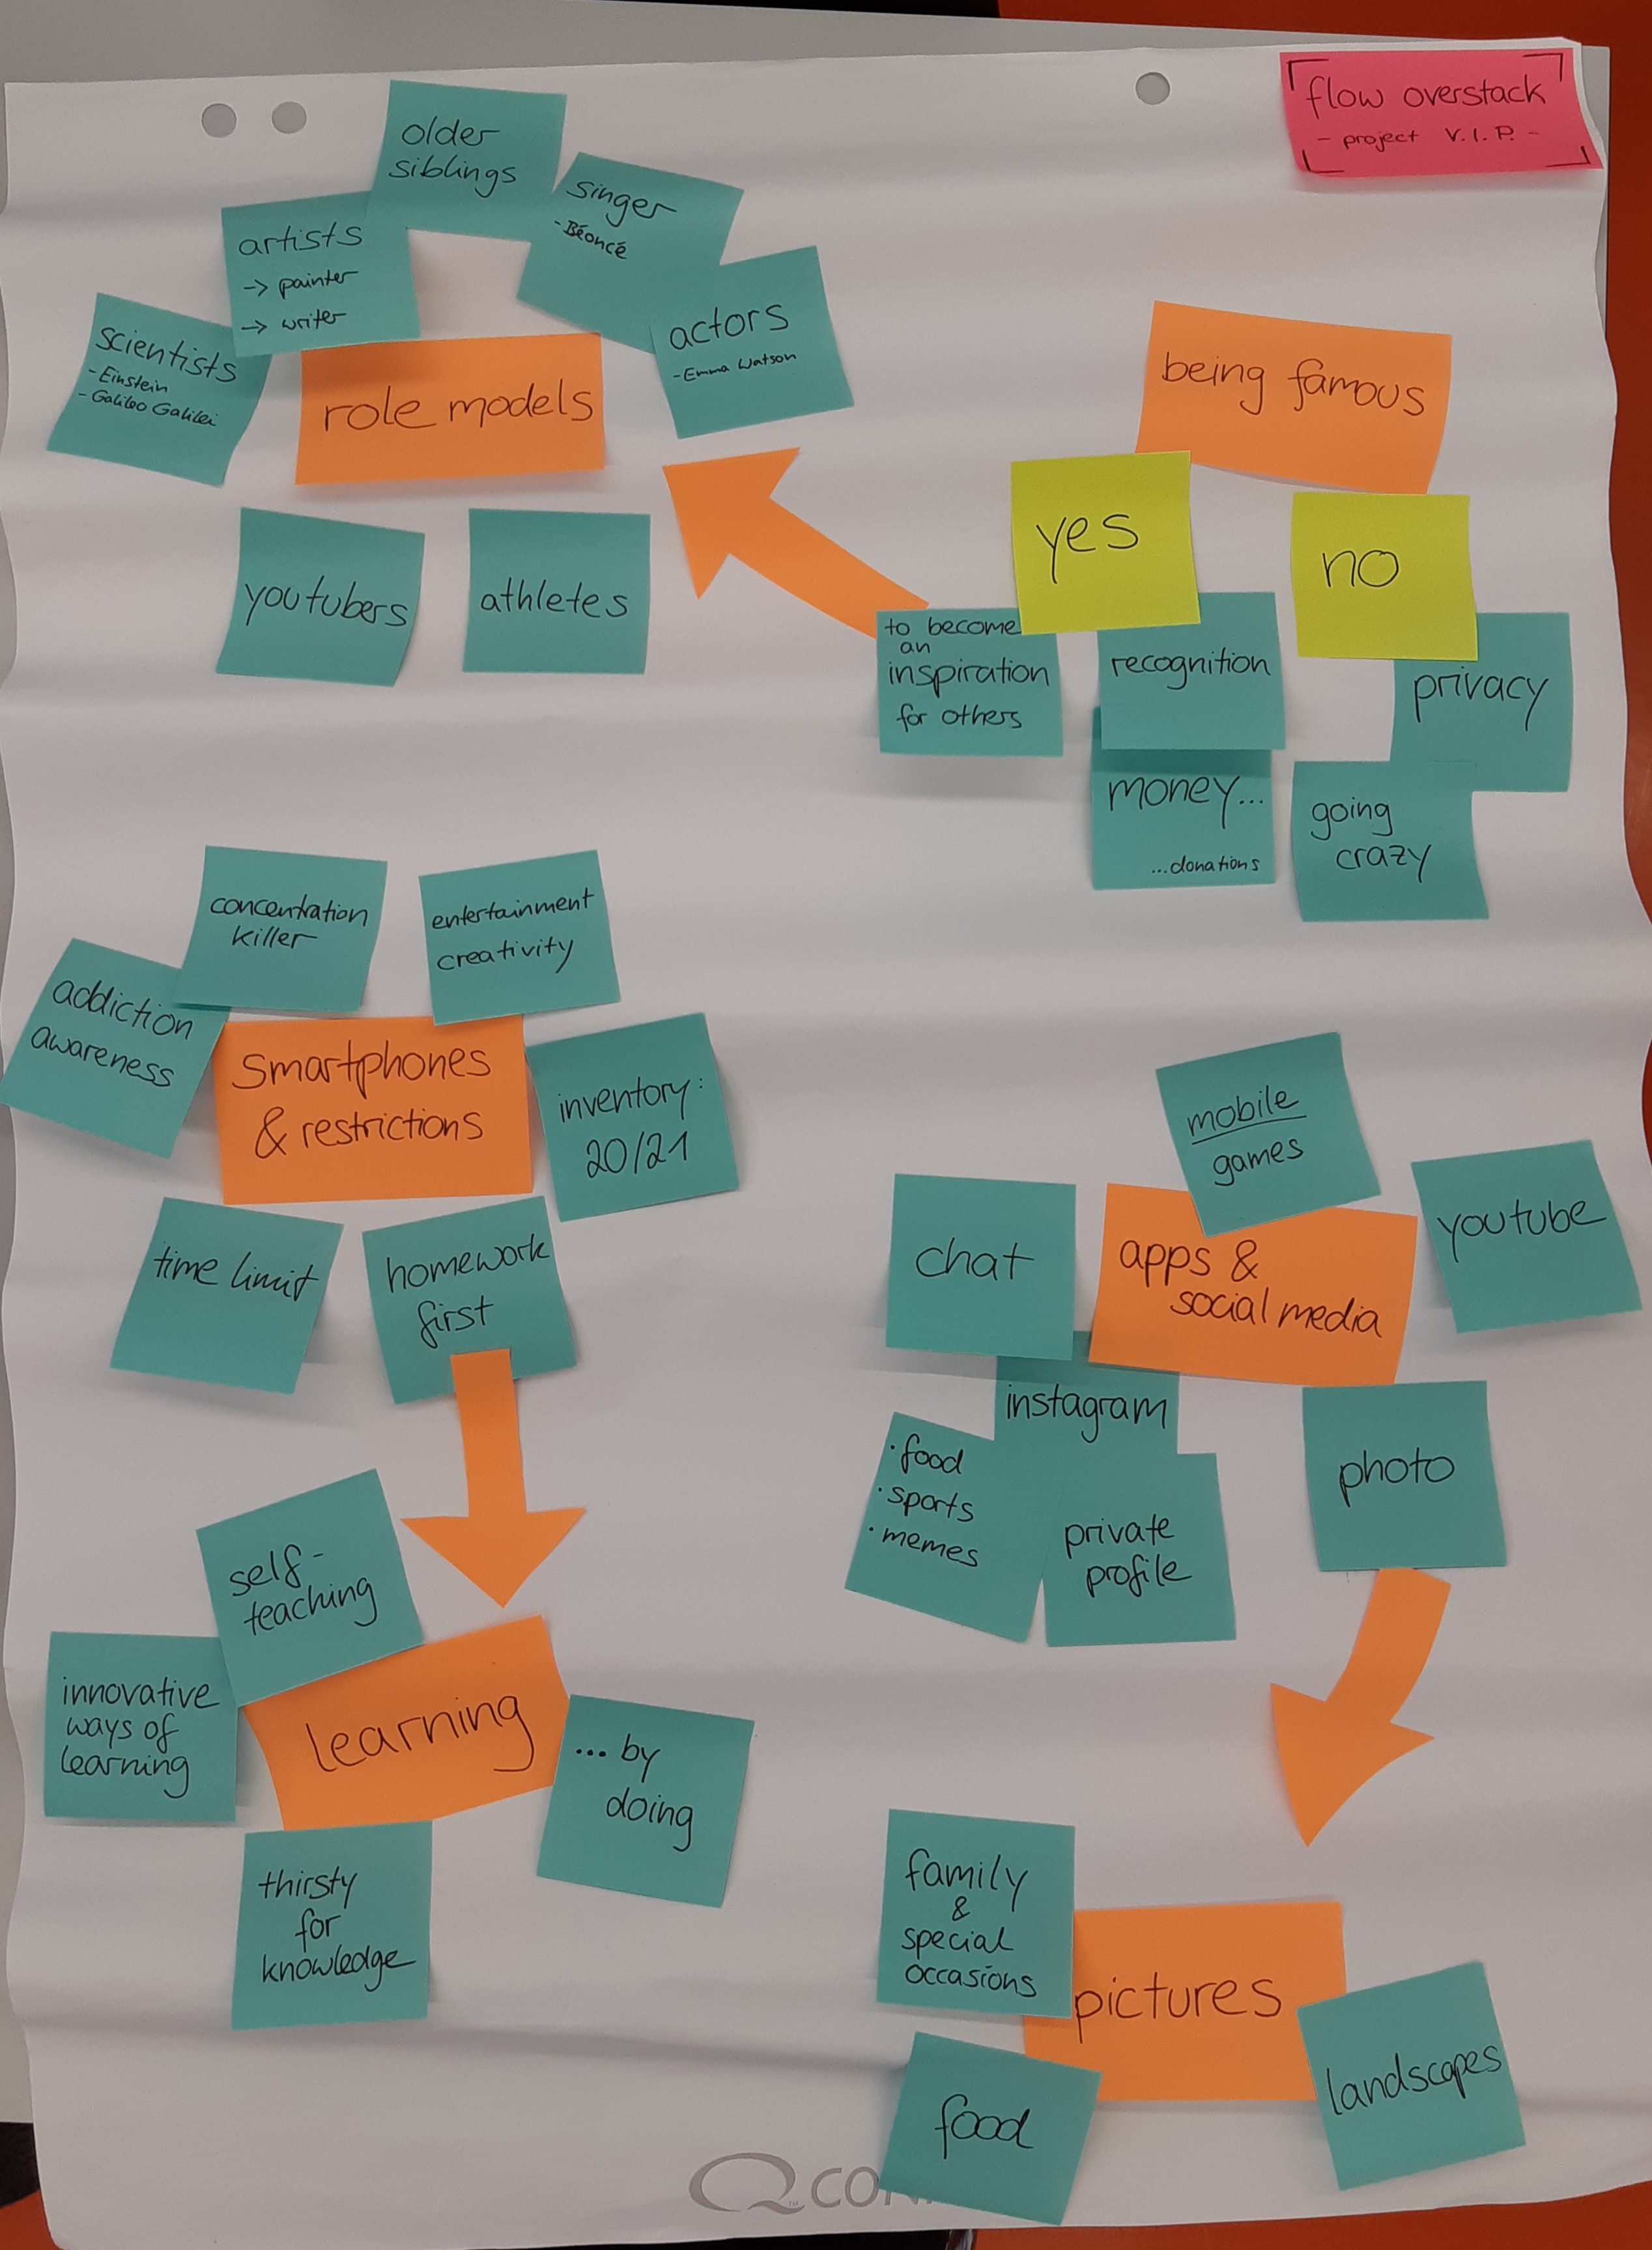
\includegraphics[width=\textwidth]{WAAD.jpg}
	\caption{The WAAD}
	\label{WAAD}
\end{figure}

\end{document}